\chapter{Observer Pattern}

\section{Định nghĩa}
Observer Pattern là một trong những Pattern thuộc nhóm hành vi (Behavior Pattern). Nó định nghĩa mối phụ thuộc một – nhiều giữa các đối tượng để khi mà một đối tượng có sự thay đổi trạng thái, tất các thành phần phụ thuộc của nó sẽ được thông báo và cập nhật một cách tự động.

\section{Mục đích sử dụng}
Mục đích và lợi ích:
\begin{itemize}
	\item	Dễ dàng mở rộng với ít sự thay đổi : mẫu này cho phép thay đổi Subject và Observer một cách độc lập. Chúng ta có thể tái sử dụng các Subject mà không cần tái sử dụng các Observer và ngược lại. Nó cho phép thêm Observer mà không sửa đổi Subject hoặc Observer khác. Vì vậy, nó đảm bảo nguyên tắc Open/Closed Principle (OCP).\\
	\item	Sự thay đổi trạng thái ở 1 đối tượng có thể được thông báo đến các đối tượng khác mà không phải giữ chúng liên kết quá chặt chẽ.\\
	\item	Một đối tượng có thể thông báo đến một số lượng không giới hạn các đối tượng khác.
\end{itemize}
Bên cạnh những lợi ích, chúng ta cần xem xét đến trường hợp cập nhật không mong muốn (Unexpected update) của Subject. Bởi vì các Observer không biết về sự hiện diện của nhau, nó có thể gây tốn nhiều chi phí của việc thay đổi Subject.
\section{Trường hợp cụ thể}
Observer Pattern được áp dụng khi:

\begin{itemize}
	\item Khi thay đổi một đối tượng, yêu cầu thay đổi đối tượng khác và chúng ta không biết có bao nhiêu đối tượng cần thay đổi, những đối tượng này là ai.\\
	\item Sử dụng trong ứng dụng broadcast-type communication.\\
	\item Sử dụng để quản lý sự kiện (Event management).\\
	\item Sử dụng trong mẫu mô hình MVC (Model View Controller Pattern) : trong MVC, mẫu này được sử dụng để tách Model khỏi View. View đại diện cho Observer và Model là đối tượng Observable.
\end{itemize}
\section{Mô hình câu trúc}
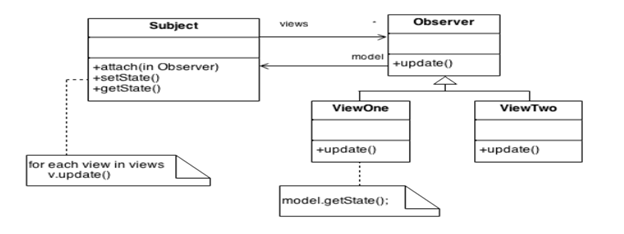
\includegraphics{GALLEYS/images/chapter2/diagram1}\\
\textbf{Subject} : cung cấp các phương thức để thêm, loại bỏ, thông báo observer.\\
\textbf{Observer} : định nghĩa một phương thức update() cho các đối tượng sẽ được subject thông báo đến khi có sự thay đổi trạng thái. \\
\textbf{ViewOne,ViewTwo ..} : có thể là bất cứ lớp con nào implement Observer interface. Mỗi observer đăng ký với một subject cụ thể để nhận được cập nhật.\\
Khi có một thay đổi nào đó, subject sẽ thông báo khi các observer có sự thay đổi. VD:
\begin{center}
	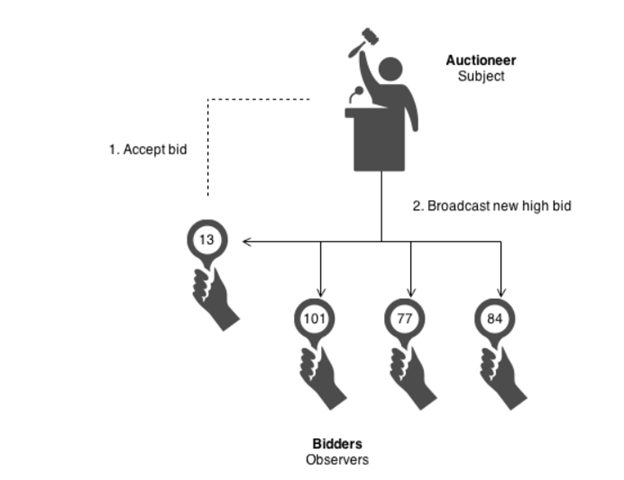
\includegraphics{GALLEYS/images/chapter2/exdiagram}\\
\end{center}
\hspace{0.5cm}Trong một cuộc đấu giá, khi một người tham gia giơ bảng giá lên,đấu giá viên bắt đầu quan sát , khi được chấp thuận, bảng giá mới sẽ được phát cho tất cả cấc nhà thầu tham gia khác.\\
   Để trực quan hơn chúng ta sẽ đến với phần ví dụ minh họa:\\
   Đây là một minh họa về trạm thời tiết Weather Station:\\

\begin{multicols}{2}
	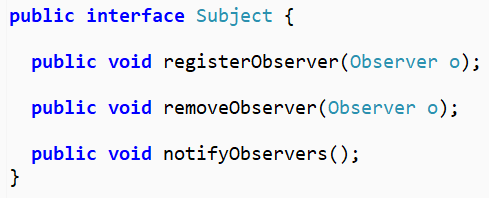
\includegraphics[width=1\columnwidth]{GALLEYS/images/chapter2/images1}\\\\\\
	Trong subject interfact có:\\
	+) public void registerObserver(Observer o) và public void removerObserver(Observer o) : cả 2 phương thức này lấy một Observer làm đối số, đó là Observer được remove hoặc register.\\
	+)phương thức notifyObservers() : phương thức này được gọi để thông báo các thành viên khi subject thay đổi.
\end{multicols}
	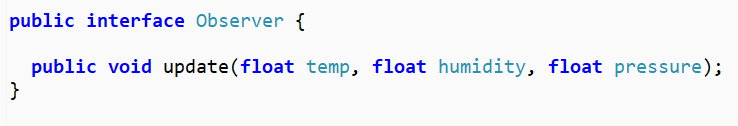
\includegraphics{GALLEYS/images/chapter2/images2}\\
	Giao diện observer được implement bởi tất cả các nhà quan sát, vì vậy tất cả phải thực hiện phương thức update() với đối số là các trạng thái mà observer nhận được khi subject đo thời tiết thay đổi.
\begin{multicols}{2}
	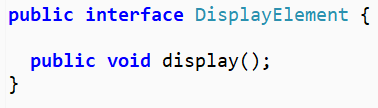
\includegraphics{GALLEYS/images/chapter2/images3}\\
	Đây là phần giao diện để hiển thị,chúng sẽ gọi phần tử hiển thị khi cần hiển thị.
\end{multicols}
\begin{multicols}{2}
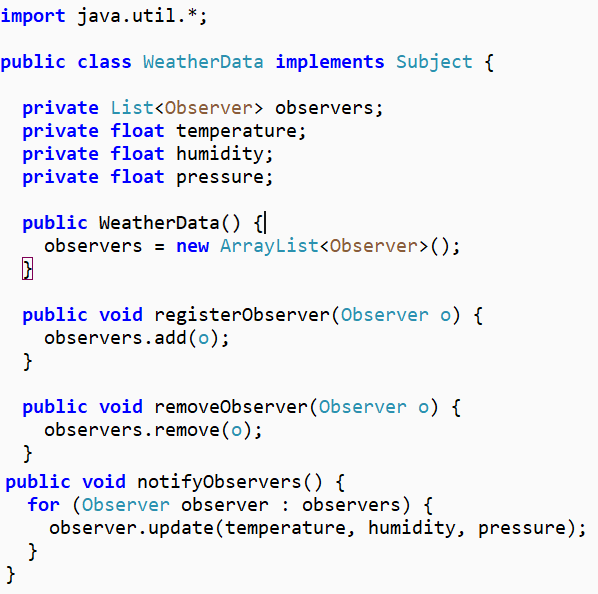
\includegraphics[width=\columnwidth]{GALLEYS/images/chapter2/images4}\\
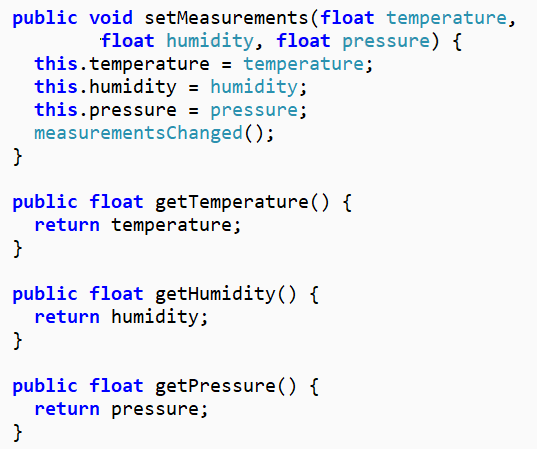
\includegraphics[width=\columnwidth]{GALLEYS/images/chapter2/images5}\\
\end{multicols}
Đây là phần chứa dữ liệu về thời tiết, lớp này được implement từ subject gồm:\\
+) có một ArrayList<Observer> (phạm vi private) dùng để lưu trữ các observer, nó được tạo ở trong construct.\\
+) các thuộc tính có bản như temperature (nhiệt độ), humidity(độ ẩm), pressure(áp suất) có phạm vi truy cập là private và kiểu dữ liệu float.\\
+) các phương thức registerObserver(Observer o) thêm các observer vào trong List khi muốn đăng ký
Phương thức removeObserver(Observer o) khi một observer muốn un-register nó sẽ xóa nó ra khỏi List\\
+) phương thức notifyObservers() sẽ thông báo update() trạng thái đến tất cả các observer\\
+) phương thức measurementsChanged() sẽ gọi đến notifyObservers() nhằm thông báo đến Observer khi có sự thay đổi phép đo.\\
+) phương thức setMeasurements() sẽ thay đổi giá trị phép đo và gọi đến measurementsChanged() nhằm thông báo đến các observers là giá trị đã thay đổi.\\
+) cuối cùng là các phương thức getTemperature() , getHumidity() và getPressure().\\
	Chúng ta sẽ đi đến phần màn hình hiển thị:\\
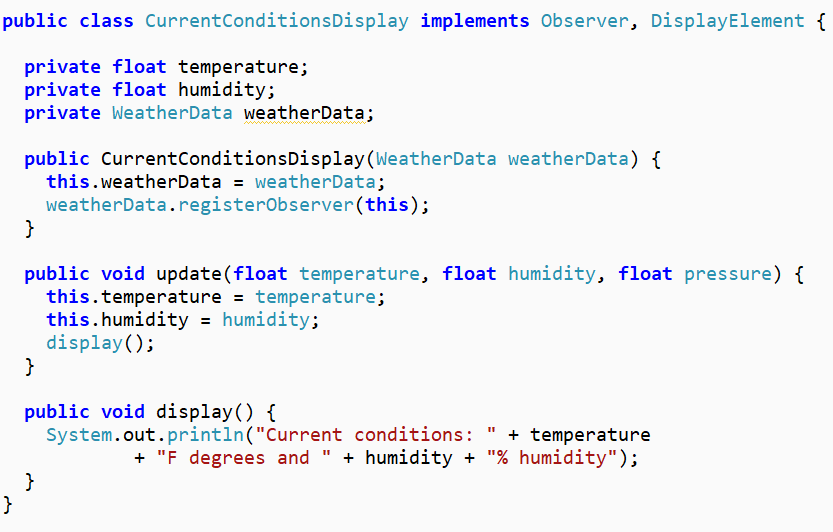
\includegraphics{GALLEYS/images/chapter2/images6}\\
Đây là màn hình thống kê và dự báo hiển thị cho nhiệt độ và độ ẩm, có một construct dùng để thông qua WeatherData và nó được dùng để đăng ký observer.
Phương thức update dùng để lưu nhiệt độ và áp suất đo được, từ đó đưa ra dự báo, khi có thay đổi . đặc biệt, WeatherData không được sử dụng, nhưng nó sẽ giúp cho việc hủy đăng ký với tư cách một observer.\\
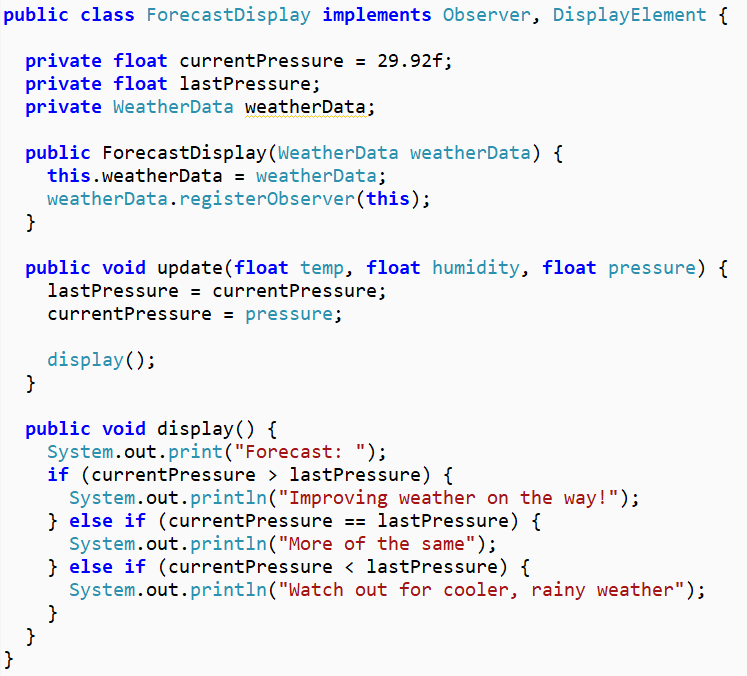
\includegraphics{GALLEYS/images/chapter2/images7}\\
Đây là màn hình thống kê và dự báo hiển thị cho áp suất chênh lệch. \\
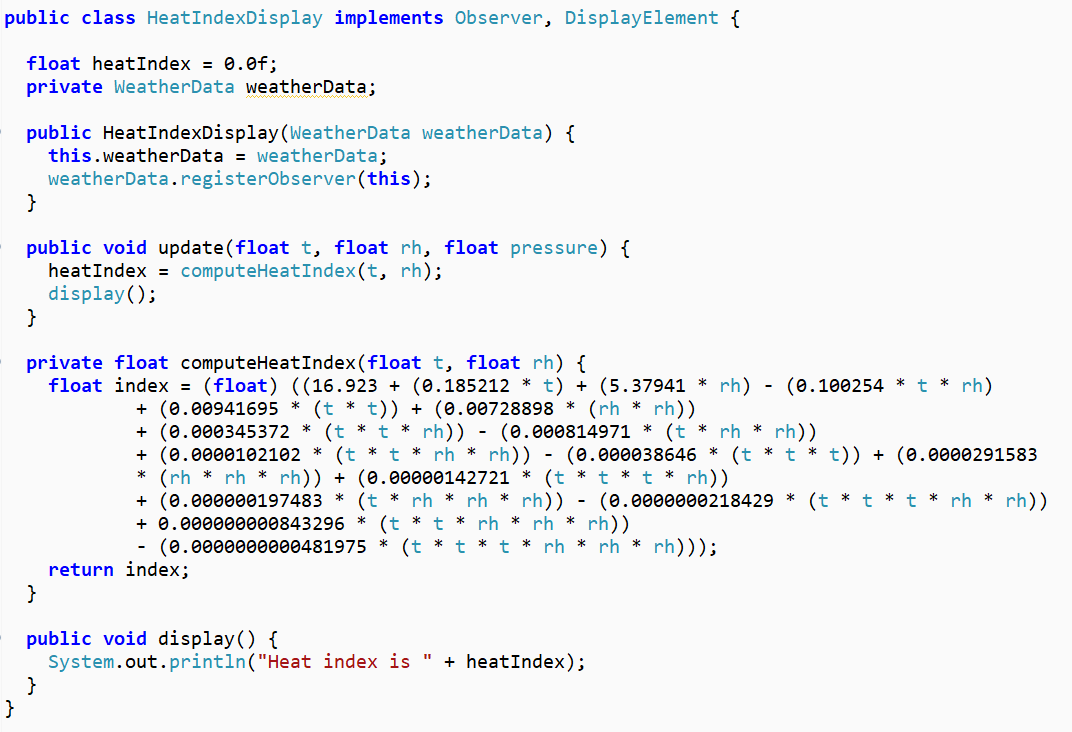
\includegraphics[width=\columnwidth,height=.45\textheight]{GALLEYS/images/chapter2/images8}\\
Đây là màn hình thống kê và dự báo hiển thị cho chỉ số nhiệt.\\\\
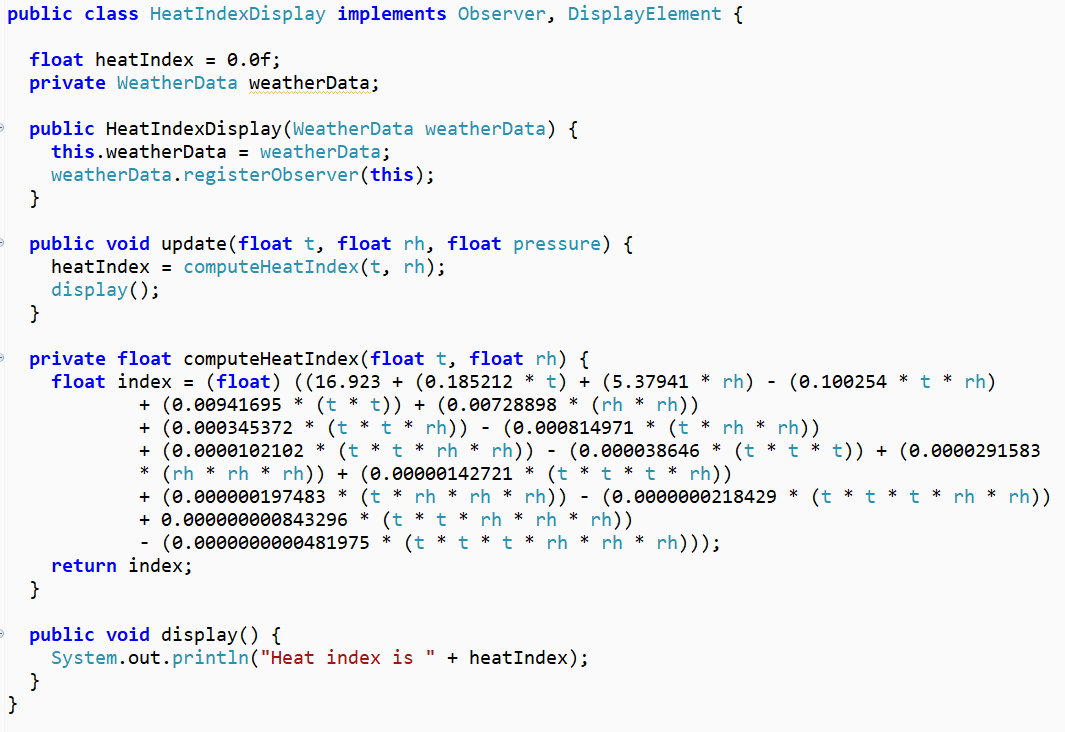
\includegraphics[width=\columnwidth,height=.5\textheight]{GALLEYS/images/chapter2/images9}\\
Đây là màn hình thống kê và dự báo hiển thị cho thống kê nhiệt độ.\\
Toàn bộ dữ liệu được thu thập từ trạm thời tiết\\
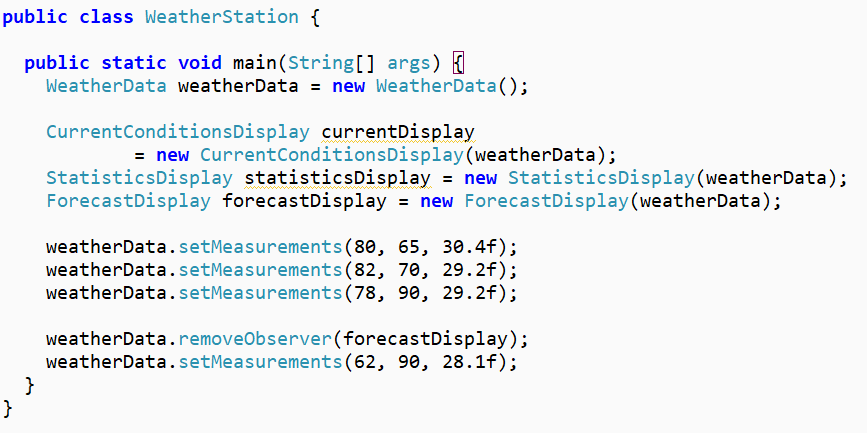
\includegraphics[width=\columnwidth,height=.4\textheight]{GALLEYS/images/chapter2/images10}\\
Trạm thời tiết sẽ hiển thi thông tin\\
Đây là kết quả:\\\\
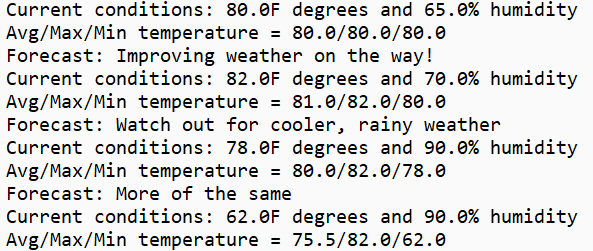
\includegraphics[width=\columnwidth,height=.3\textheight]{GALLEYS/images/chapter2/images11}\\\\
Mẫu thiết kế Observer (quan sát) có thể được sử dụng bất cứ khi nào mà một đối tượng có sự thay đổi trạng thái, tất các thành phần phụ thuộc của nó sẽ được thông báo và cập nhật một cách tự động.\\


